%
% This document contains the chapter about DC analysis.
%
% Copyright (C) 2003, 2004, 2005, 2006 Stefan Jahn <stefan@lkcc.org>
% Copyright (C) 2004 Michael Margraf <Michael.Margraf@alumni.TU-Berlin.DE>
%
% Permission is granted to copy, distribute and/or modify this document
% under the terms of the GNU Free Documentation License, Version 1.1
% or any later version published by the Free Software Foundation.
%

\chapter{DC Analysis}
%\addcontentsline{toc}{chapter}{DC Analysis}

\section{Modified Nodal Analysis}
%\addcontentsline{toc}{section}{Modified Nodal Analysis}
\label{sec:MNA}

Many different kinds of network element are encountered in network
analysis.  For circuit analysis it is necessary to formulate equations
for circuits containing as many different types of network elements as
possible.  There are various methods for equation formulation for a
circuit.  These are based on three types of equations found in circuit
theory:

\begin{itemize}
\item equations based on Kirchhoff's voltage law (KVL)
\item equations based on Kirchhoff's current law (KCL)
\item branch constitutive equations
\end{itemize}

The equations have to be formulated (represented in a computer
program) automatically in a simple, comprehensive manner.  Once
formulated, the system of equations has to be solved.  There are two
main aspects to be considered when choosing algorithms for this
purpose: accuracy and speed.  The MNA, briefly for \textbf{M}odified
\textbf{N}odal \textbf{A}nalysis, has been proved to accomplish these
tasks.

MNA applied to a circuit with passive elements, independent current
and voltage sources and active elements results in a matrix equation
of the form:
\begin{equation}
\left[A\right] \cdot \left[x\right] = \left[z\right]
\end{equation}

For a circuit with N nodes and M independent voltage sources:

\begin{itemize}

\item The A matrix
\begin{itemize}
\item
is (N+M)$\times$(N+M) in size, and consists only of known quantities
\item
the N$\times$N part of the matrix in the upper left:
\begin{itemize}
\item
has only passive elements
\item
elements connected to ground appear only on the diagonal
\item
elements not connected to ground are both on the diagonal and
off-diagonal terms
\end{itemize}
\item
the rest of the A matrix (not included in the N$\times$N upper left
part) contains only 1, -1 and 0 (other values are possible if there
are dependent current and voltage sources)
\end{itemize}

\item The x matrix
\begin{itemize}
\item
is an (N+M)$\times$1 vector that holds the unknown quantities (node
voltages and the currents through the independent voltage sources)
\item
the top N elements are the n node voltages
\item
the bottom M elements represent the currents through the M independent
voltage sources in the circuit
\end{itemize}

\item The z matrix
\begin{itemize}
\item
is an (N+M)$\times$1 vector that holds only known quantities
\item
the top N elements are either zero or the sum and difference of
independent current sources in the circuit
\item
the bottom M elements represent the M independent voltage sources in
the circuit
\end{itemize}
\end{itemize}

The circuit is solved by a simple matrix manipulation:
\begin{equation}
\left[x\right] = \left[A\right]^{-1} \cdot \left[z\right]
\end{equation}

Though this may be difficult by hand, it is straightforward and so is
easily done by computer.

\subsection{Generating the MNA matrices}
%\addcontentsline{toc}{subsection}{Generating the MNA matrices}

The following section is an algorithmic approach to the concept of the
Modified Nodal Analysis.  There are three matrices we need to
generate, the A matrix, the x matrix and the z matrix.  Each of these
will be created by combining several individual sub-matrices.

\subsection{The A matrix}
%\addcontentsline{toc}{subsection}{The A matrix}

The A matrix will be developed as the combination of 4 smaller
matrices, G, B, C, and D.

\begin{equation}
A =
\begin{bmatrix}
G & B\\
C & D
\end{bmatrix}
\end{equation}

The A matrix is (M+N)$\times$(M+N) (N is the number of nodes, and M is the
number of independent voltage sources) and:

\begin{itemize}
\item
the G matrix is N$\times$N and is determined by the interconnections
between the circuit elements
\item
the B matrix is N$\times$M and is determined by the connection of the voltage
sources
\item
the C matrix is M$\times$N and is determined by the connection of
the voltage sources (B and C are closely related, particularly when
only independent sources are considered)
\item
the D matrix is M$\times$M and is zero if only independent sources are
considered
\end{itemize}

\subsubsection{Rules for making the G matrix}
%\addcontentsline{toc}{subsubsection}{Rules for making the G matrix}

The G matrix is an N$\times$N matrix formed in two steps.

\begin{enumerate}
\item
Each element in the diagonal matrix is equal to the sum of the
conductance (one over the resistance) of each element connected to the
corresponding node.  So the first diagonal element is the sum of
conductances connected to node 1, the second diagonal element is the
sum of conductances connected to node 2, and so on.
\item
The off diagonal elements are the negative conductance of the element
connected to the pair of corresponding node.  Therefore a resistor
between nodes 1 and 2 goes into the G matrix at location (1,2) and
locations (2,1).
\end{enumerate}

If an element is grounded, it will only have contribute to one entry
in the G matrix -- at the appropriate location on the diagonal.  If it
is ungrounded it will contribute to four entries in the matrix -- two
diagonal entries (corresponding to the two nodes) and two off-diagonal
entries.

\subsubsection{Rules for making the B matrix}
%\addcontentsline{toc}{subsubsection}{Rules for making the B matrix}

The B matrix is an N$\times$M matrix with only 0, 1 and -1 elements.
Each location in the matrix corresponds to a particular voltage source
(first dimension) or a node (second dimension).  If the positive
terminal of the ith voltage source is connected to node k, then the
element (k,i) in the B matrix is a 1.  If the negative terminal of the
ith voltage source is connected to node k, then the element (k,i) in
the B matrix is a -1.  Otherwise, elements of the B matrix are zero.

\addvspace{12pt}

If a voltage source is ungrounded, it will have two elements in the B
matrix (a 1 and a -1 in the same column).  If it is grounded it will
only have one element in the matrix.

\subsubsection{Rules for making the C matrix}
%\addcontentsline{toc}{subsubsection}{Rules for making the C matrix}

The C matrix is an M$\times$N matrix with only 0, 1 and -1 elements.
Each location in the matrix corresponds to a particular node (first
dimension) or voltage source (second dimension).  If the positive
terminal of the ith voltage source is connected to node k, then the
element (i,k) in the C matrix is a 1.  If the negative terminal of the
ith voltage source is connected to node k, then the element (i,k) in
the C matrix is a -1.  Otherwise, elements of the C matrix are zero.

\addvspace{12pt}

In other words, the C matrix is the transpose of the B matrix.  This
is not the case when dependent sources are present.

\subsubsection{Rules for making the D matrix}
%\addcontentsline{toc}{subsubsection}{Rules for making the D matrix}

The D matrix is an M$\times$M matrix that is composed entirely of
zeros.  It can be non-zero if dependent sources are considered.

\subsection{The x matrix}
\label{sec:xmatrix}
%\addcontentsline{toc}{subsection}{The x matrix}

The x matrix holds our unknown quantities and will be developed as the
combination of 2 smaller matrices v and j.  It is considerably easier
to define than the A matrix.

\begin{equation}
x =
\begin{bmatrix}
v\\
j
\end{bmatrix}
\end{equation}

The x matrix is 1$\times$(M+N) (N is the number of nodes, and M is the
number of independent voltage sources) and:

\begin{itemize}
\item
the v matrix is 1$\times$N and hold the unknown voltages
\item
the j matrix is 1$\times$M and holds the unknown currents through the
voltage sources
\end{itemize}

\subsubsection{Rules for making the v matrix}
%\addcontentsline{toc}{subsubsection}{Rules for making the v matrix}

The v matrix is an 1$\times$N matrix formed of the node voltages.
Each element in v corresponds to the voltage at the equivalent node in
the circuit (there is no entry for ground -- node 0).

\addvspace{12pt}

For a circuit with N nodes we get:

\begin{equation}
v =
\begin{bmatrix}
v_{1}\\
v_{2}\\
\vdots\\
v_{N}\\
\end{bmatrix}
\end{equation}

\subsubsection{Rules for making the j matrix}
%\addcontentsline{toc}{subsubsection}{Rules for making the j matrix}

The j matrix is an 1$\times$M matrix, with one entry for the current
through each voltage source.  So if there are M voltage sources
$V_{1}$, $V_{2}$ through $V_{M}$, the j matrix will be:

\begin{equation}
j =
\begin{bmatrix}
i_{V_{1}}\\
i_{V_{2}}\\
\vdots\\
i_{V_{M}}\\
\end{bmatrix}
\end{equation}

\subsection{The z matrix}
%\addcontentsline{toc}{subsection}{The z matrix}

The z matrix holds our independent voltage and current sources and
will be developed as the combination of 2 smaller matrices i and e.
It is quite easy to formulate.

\begin{equation}
z =
\begin{bmatrix}
i\\
e
\end{bmatrix}
\end{equation}

The z matrix is 1$\times$(M+N) (N is the number of nodes, and M is the
number of independent voltage sources) and:

\begin{itemize}
\item
the i matrix is 1$\times$N and contains the sum of the currents through the
passive elements into the corresponding node (either zero, or the sum
of independent current sources)
\item
the e matrix is 1$\times$M and holds the values of the independent
voltage sources
\end{itemize}

\subsubsection{Rules for making the i matrix}
%\addcontentsline{toc}{subsubsection}{Rules for making the i matrix}

The i matrix is an 1$\times$N matrix with each element of the matrix
corresponding to a particular node.  The value of each element of i is
determined by the sum of current sources into the corresponding node.
If there are no current sources connected to the node, the value is
zero.

\subsubsection{Rules for making the e matrix}
%\addcontentsline{toc}{subsubsection}{Rules for making the e matrix}

The e matrix is an 1$\times$M matrix with each element of the matrix
equal in value to the corresponding independent voltage source.

\subsection{A simple example}
%\addcontentsline{toc}{subsection}{A simple example}

The example given in fig. \ref{fig:MNAexample} illustrates applying
the rules for building the MNA matrices and how this relates to basic
equations used in circuit analysis.

\begin{figure}[ht]
\begin{center}
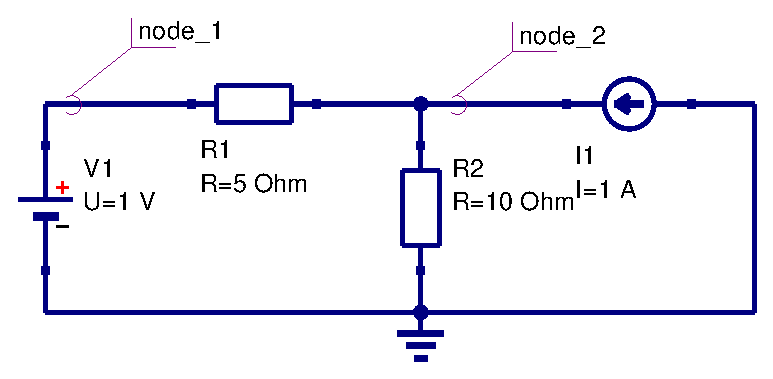
\includegraphics[width=10cm]{MNAexample}
\end{center}
\caption{example circuit applied to modified nodal analysis}
\label{fig:MNAexample}
\end{figure}
\FloatBarrier

\subsubsection{Going through the MNA algorithm}
%\addcontentsline{toc}{subsubsection}{Going through the MNA algorithm}

The G matrix is a 2$\times$2 matrix because there are 2 different
nodes apart from ground which is the reference node.  On the diagonal
you find the sum of the elements conductances connected to the nodes 1
and 2.  The off-diagonal matrix entries contain the negative
conductances of the elements connected between two nodes.

\begin{equation}
G =
\begin{bmatrix}
\frac{1}{R_{1}} & -\frac{1}{R_{1}}\\
-\frac{1}{R_{1}} & \frac{1}{R_{1}} + \frac{1}{R_{2}}
\end{bmatrix}
=
\begin{bmatrix}
0.2 & -0.2\\
-0.2 & 0.3
\end{bmatrix}
\end{equation}

The B matrix (which is transposed to C) is a 1$\times$2 matrix because
there is one voltage source and 2 nodes.  The positive terminal of the
voltage source $V_{1}$ is connected to node 1.  That is why

\begin{equation}
B = C^{T} =
\begin{bmatrix}
1\\
0
\end{bmatrix}
\end{equation}

and the D matrix is filled with zeros only because there are no dependent
(active and controlled) devices in the example circuit.

\begin{equation}
D =
\begin{bmatrix}
0
\end{bmatrix}
\end{equation}

The x matrix is a 1$\times$3 matrix.  The MNA equations deliver a
solution for the unknown voltages at each node in a circuit except the
reference node and the currents through each voltage source.

\begin{equation}
x =
\begin{bmatrix}
v_{1}\\
v_{2}\\
i_{V_{1}}
\end{bmatrix}
\end{equation}

The z matrix is according to the rules for building it a 1$\times$3
matrix.  The upper two entries are the sums of the currents flowing
into node 1 and node 2.  The lower entry is the voltage value of the
voltage source $V_{1}$.

\begin{equation}
z =
\begin{bmatrix}
0\\
I_{1}\\
U_{1}
\end{bmatrix}
=
\begin{bmatrix}
0\\
1\\
1
\end{bmatrix}
\end{equation}

According to the MNA algorithm the equation system is represented by

\begin{equation}
\left[A\right] \cdot \left[x\right] = \left[z\right]
\end{equation}

which is equivalent to

\begin{equation}
\begin{bmatrix}
G & B\\
C & D
\end{bmatrix}
\cdot
\begin{bmatrix}
x
\end{bmatrix}
=
\begin{bmatrix}
z
\end{bmatrix}
\label{eq:MNAexample}
\end{equation}

In the example eq. \eqref{eq:MNAexample} expands to:

\begin{equation}
\begin{bmatrix}
\frac{1}{R_{1}} & -\frac{1}{R_{1}} & 1\\
-\frac{1}{R_{1}} & \frac{1}{R_{1}} + \frac{1}{R_{2}} & 0\\
1 & 0 & 0
\end{bmatrix}
\cdot
\begin{bmatrix}
v_{1}\\
v_{2}\\
i_{V_{1}}
\end{bmatrix}
=
\begin{bmatrix}
0\\
I_{1}\\
U_{1}
\end{bmatrix}
\label{eq:MNAfull}
\end{equation}

The equation systems to be solved is now defined by the following
matrix representation.

\begin{equation}
\begin{bmatrix}
0.2 & -0.2 & 1\\
-0.2 & 0.3 & 0\\
1 & 0 & 0
\end{bmatrix}
\cdot
\begin{bmatrix}
v_{1}\\
v_{2}\\
i_{V_{1}}
\end{bmatrix}
=
\begin{bmatrix}
0\\
1\\
1
\end{bmatrix}
\end{equation}

Using matrix inversion the solution vector x writes as follows:

\begin{equation}
\left[x\right] = 
\left[A\right]^{-1}\cdot \left[z\right] = 
\begin{bmatrix}
v_{1}\\
v_{2}\\
i_{V_{1}}
\end{bmatrix}
=
\begin{bmatrix}
1\\
4\\
0.6
\end{bmatrix}
\label{eq:MNAresult}
\end{equation}

The result in eq. (\ref{eq:MNAresult}) denotes the current through the
voltage source $V_{1}$ is $0.6\ampere$, the voltage at node 1 is
$1\volt$ and the voltage at node 2 is $4\volt$.

\subsubsection{How the algorithm relates to basic equations in circuit analysis}
%\addcontentsline{toc}{subsubsection}{How the algorithm relates to basic equations in circuit analysis}

Expanding the matrix representation in eq. (\ref{eq:MNAfull}) to a set
of equations denotes the following equation system consisting of 3 of
them.

\begin{align}
\rm{I:}& \qquad 0 = \frac{1}{R_{1}}\cdot v_{1} - \frac{1}{R_{1}}\cdot v_{2} + i_{V_{1}}& \text{KCL at node 1}\\
\rm{II:}& \qquad I_{1} = -\frac{1}{R_{1}}\cdot v_{1} + \left(\frac{1}{R_{1}} + \frac{1}{R_{2}}\right)\cdot v_{2}& \text{KCL at node 2}\\
\rm{III:}& \qquad U_{1} = v_{1}& \text{constitutive equation}
\end{align}

Apparently eq. I and eq. II conform to Kirchhoff's current law at the
nodes 1 and 2.  The last equation is just the constitutive equation
for the voltage source $V_{1}$.  There are three unknowns ($v_{1}$,
$v_{2}$ and $i_{V_{1}}$) and three equations, thus the system should
be solvable.

\addvspace{12pt}

Equation III indicates the voltage at node 1 is $1\volt$.  Applying
this result to eq. II and transposing it to $v_{2}$ (the voltage at
node 2) gives

\begin{equation}
v_{2} = \frac{I_{1} + \frac{1}{R_{1}}\cdot U_{1}}{\frac{1}{R_{1}} + \frac{1}{R_{2}}} = 4\volt
\end{equation}

The missing current through the voltage source $V_{1}$ can be computed
using both the results $v_{2} = 4\volt$ and $v_{1} = 1\volt$ by
transforming equation I.

\begin{equation}
i_{V_{1}} = \frac{1}{R_{1}}\cdot v_{2} - \frac{1}{R_{1}}\cdot v_{1} = 0.6\ampere
\end{equation}

The small example, shown in fig. \ref{fig:MNAexample}, and the
excursus into artless math verifies that the MNA algorithm and classic
electrical handiwork tend to produce the same results.

\section{Extensions to the MNA}
%\addcontentsline{toc}{section}{Extensions to the MNA}
\label{sec:MNAext}

As noted in the previous sections the D matrix is zero and the B and C
matrices are transposed each other and filled with either 1, -1 or 0
provided that there are no dependent sources within the circuit.  This
changes when introducing active (and controlled) elements. Examples
are voltage controlled voltage sources, transformers and ideal
operational amplifiers. The models are depicted in section
\ref{sec:NLdevices} and \ref{sec:Ldevices}


\section{Non-linear DC Analysis}
%\addcontentsline{toc}{section}{Non-linear DC Analysis}

Previous sections described using the modified nodal analysis solving
linear networks including controlled sources.  It can also be used to
solve networks with non-linear components like diodes and transistors.
Most methods are based on iterative solutions of a linearised equation
system.  The best known is the so called Newton-Raphson method.

\subsection{Newton-Raphson method}
%\addcontentsline{toc}{subsection}{Newton-Raphson method}
\label{sec:NRmethod}

The Newton-Raphson method is going to be introduced using the example
circuit shown in fig. \ref{fig:NLexample} having a single unknown: the
voltage at node 1.

\begin{figure}[ht]
\begin{center}
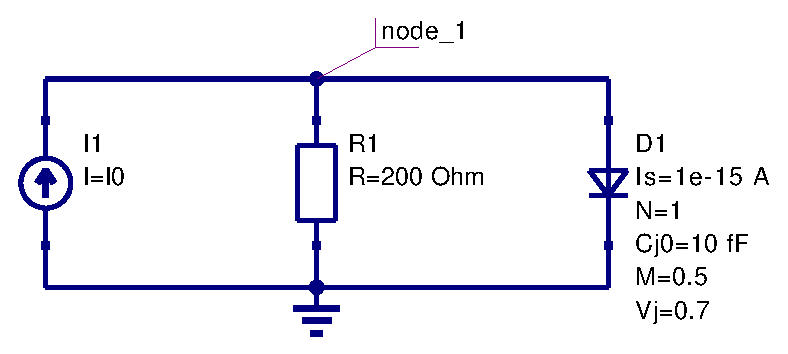
\includegraphics[width=10cm]{NLexample}
\end{center}
\caption{example circuit for non-linear DC analysis}
\label{fig:NLexample}
\end{figure}
\FloatBarrier

The 1x1 MNA equation system to be solved can be written as
\begin{equation}
\begin{bmatrix}
G
\end{bmatrix}
\cdot
\begin{bmatrix}
V_{1}
\end{bmatrix}
=
\begin{bmatrix}
I_{0}
\end{bmatrix}
\label{eq:NLmatrix}
\end{equation}

whereas the value for $G$ is now going to be explained.  The current
through a diode is simply determined by Schockley's approximation
\begin{equation}
I_{d} = I_{S}\cdot \left(e^{\frac{V_{d}}{V_{T}}} - 1\right)
\end{equation}

Thus Kirchhoff's current law at node 1 can be expressed as
\begin{equation}
I_{0} = \dfrac{V}{R} + I_{S}\cdot \left(e^{\frac{V}{V_{T}}} - 1\right)
\end{equation}

By establishing eq. (\ref{eq:NLfunc}) it is possible to trace the
problem back to finding the zero point of the function $f$.
\begin{equation}
f(V) = \dfrac{V}{R} + I_{S}\cdot \left(e^{\frac{V}{V_{T}}} - 1\right) - I_{0}
\label{eq:NLfunc}
\end{equation}

Newton developed a method stating that the zero point of a functions
derivative (i.e. the tangent) at a given point is nearer to the zero
point of the function itself than the original point.  In mathematical
terms this means to linearise the function $f$ at a starting value
$V^{(0)}$.
\begin{equation}
f\left(V^{(0)} + \Delta V\right) \approx f\left(V^{(0)}\right) + \left.\dfrac{\partial f\left(V\right)}{\partial V}\right|_{V^{(0)}}\cdot \Delta V
\;\;\;\; \text{ with } \;\;\;\;
\Delta V = V^{(1)} - V^{(0)}
\label{eq:NRapprox}
\end{equation}

Setting $f(V^{(1)}) = 0$ gives
\begin{equation}
V^{(1)} = V^{(0)} - \dfrac{f\left(V^{(0)}\right)}{\left.\dfrac{\partial f\left(V\right)}{\partial V}\right|_{V^{(0)}}}
\end{equation}

or in the general case with $m$ being the number of iteration
\begin{equation}
V^{(m + 1)} = V^{(m)} - \dfrac{f\left(V^{(m)}\right)}{\left.\dfrac{\partial f\left(V\right)}{\partial V}\right|_{V^{(m)}}}
\label{eq:NRgeneral}
\end{equation}

This must be computed until $V^{(m+1)}$ and $V^{(m)}$ differ less than a
certain barrier.
\begin{equation}
\left|V^{(m+1)} - V^{(m)}\right| < \varepsilon_{abs} + \varepsilon_{rel}\cdot \left|V^{(m)}\right|
\label{eq:NLconvergence}
\end{equation}

With very small $\varepsilon_{abs}$ the iteration would break too
early and for little $\varepsilon_{rel}$ values the iteration aims to
a useless precision for large absolute values of $V$.

\begin{figure}[ht]
\begin{center}
\psfrag{V0}{$\mathrm{V^{(0)}}$}
\psfrag{V1}{$\mathrm{V^{(1)}}$}
\psfrag{V2}{$\mathrm{V^{(2)}}$}
\includegraphics[width=0.75\linewidth]{newton}
\end{center}
\caption{Newton-Raphson method for example circuit}
\label{fig:NewtonRaphson}
\end{figure}
\FloatBarrier

With this theoretical background it is now possible to step back to
eq. (\ref{eq:NLfunc}) being the determining equation for the example
circuit.  With
\begin{equation}
g_{d}^{(m)} = \left.\dfrac{\partial I_{d}}{\partial V}\right|_{V^{(m)}} = \dfrac{I_{S}}{V_{T}}\cdot e^{\frac{V^{(m)}}{V_{T}}}
\end{equation}

and
\begin{equation}
\left.\dfrac{\partial f\left(V\right)}{\partial V}\right|_{V^{(m)}} = \dfrac{1}{R} + g_{d}^{(m)}
\end{equation}

the eq. (\ref{eq:NRgeneral}) can be written as
\begin{equation}
\left(g_{d}^{(m)} + \dfrac{1}{R}\right)\cdot V^{(m+1)} = I_{0} - \left(I_{d}^{(m)} - g_{d}^{(m)}\cdot V^{(m)}\right)
\label{eq:NRresult}
\end{equation}

when the expression
\begin{equation}
f\left(V^{(m)}\right) = \dfrac{1}{R}\cdot V^{(m)} + I_{d}^{(m)} - I_{0}
\end{equation}

based upon eq. (\ref{eq:NLfunc}) is taken into account.  Comparing the
introductory MNA equation system in eq. (\ref{eq:NLmatrix}) with
eq. (\ref{eq:NRresult}) proposes the following equivalent circuit for
the diode model.

\begin{figure}[ht]
\begin{center}
\psfrag{gd}{$\mathrm{g_{d}^{(m)}}$}
\psfrag{Ieq}{$\mathrm{I_{d}^{(m)} - g_{d}^{(m)}\cdot V^{(m)}}$}
\includegraphics[width=0.2\linewidth]{newtondiode}
\end{center}
\caption{accompanied equivalent circuit for intrinsic diode}
\label{fig:AccompaniedModel}
\end{figure}
\FloatBarrier

\label{sec:DCdiode}

With
\begin{equation}
I_{eq} = I_{d}^{(m)} - g_{d}^{(m)}\cdot V^{(m)}
\end{equation}

the MNA matrix entries can finally be written as
\begin{equation}
\begin{bmatrix}
g_{d} & -g_{d}\\
-g_{d} & g_{d}
\end{bmatrix}
\cdot
\begin{bmatrix}
V_{1}\\
V_{2}
\end{bmatrix}
=
\begin{bmatrix}
-I_{eq}\\
I_{eq}
\end{bmatrix}
\end{equation}

In analog ways all controlled current sources with non-linear
current-voltage dependency built into diodes and transistors can be
modeled.  The left hand side of the MNA matrix (the A matrix) is
called Jacobian matrix which is going to be build in each iteration
step.  For the solution vector $x$ possibly containing currents as
well when voltage sources are in place a likely convergence criteria
as defined in eq. (\ref{eq:NLconvergence}) must be defined for the
currents.

\addvspace{12pt}

Having understood the one-dimensional example, it is now only a
small step to the general multi-dimensional algorithm: The node
voltage becomes a vector $\boldsymbol{V}^{(m)}$, factors become
the corresponding matrices and differentiations become Jacobian
matrices.

\addvspace{12pt}

The function whose zero must be found is the transformed MNA
equation \ref{eq:NLmatrix}:

\begin{equation}
\boldsymbol{f}( \boldsymbol{V}^{(m)} ) =
    \boldsymbol{G}\cdot \boldsymbol{V}^{(m)} - \boldsymbol{I}_{0}^{(m)}
\end{equation}

The only difference to the linear case is that the vector $\boldsymbol{I}_{0}$
also contains the currents flowing out of the non-linear components.
The iteration formula of the Newton-Raphson method writes:

\begin{equation}
\boldsymbol{V}^{(m+1)} = \boldsymbol{V}^{(m)} -
  \left( \left.\frac{\partial\boldsymbol{f}( \boldsymbol{V} )}
                    {\partial\boldsymbol{V}}\right|_{V^{(m)}} \right)^{-1}
  \cdot \boldsymbol{f}( \boldsymbol{V}^{(m)} )
\label{eq:ndimNewton}
\end{equation}

Note that the Jacobian matrix is nothing else but the real
part of the MNA matrix for the AC analysis:

\begin{equation}
\boldsymbol{J}^{(m)}
  = \left.\frac{\partial\boldsymbol{f}( \boldsymbol{V} )}
               {\partial\boldsymbol{V}}\right|_{\boldsymbol{V}^{(m)}}
  = \boldsymbol{G} - \left.\frac{\partial\boldsymbol{I}_{0}}
               {\partial\boldsymbol{V}}\right|_{\boldsymbol{V}^{(m)}}
  = \boldsymbol{G} - \boldsymbol{J}_{nl}^{(m)}
  = \text{Re}\left(\boldsymbol{G}_{AC}\right)
\label{eq:ndimJacobi}
\end{equation}

where the index $nl$ denotes only the non-linear terms. Putting equation
\ref{eq:ndimJacobi} into equation \ref{eq:ndimNewton} and multiplying it
with the Jacobian matrix leads to

\begin{align}
\boldsymbol{J}^{(m)} \cdot \boldsymbol{V}^{(m+1)}
 &= \boldsymbol{J}^{(m)} \cdot \boldsymbol{V}^{(m)} -
    \boldsymbol{f}( \boldsymbol{V}^{(m)} ) \\
 &= \left( \boldsymbol{G} - \boldsymbol{J}_{nl}^{(m)} \right) \cdot \boldsymbol{V}^{(m)} -
    \boldsymbol{G} \cdot \boldsymbol{V}^{(m)} + \boldsymbol{I}_{0}^{(m)} \\
 &= -\boldsymbol{J}_{nl}^{(m)} \cdot \boldsymbol{V}^{(m)} + \boldsymbol{I}_{0}^{(m)}
\end{align}

So, bringing the Jacobian back to the right side results in the new
iteration formula:

\begin{equation}
\boldsymbol{V}^{(m+1)} = \left( \boldsymbol{J}^{(m)} \right)^{-1} \cdot
  \left( -\boldsymbol{J}_{nl}^{(m)}\cdot \boldsymbol{V}^{(m)} + \boldsymbol{I}_{0}^{(m)} \right)
\end{equation}

The negative sign in front of $\boldsymbol{J}_{nl}$ is due to the
definition of $\boldsymbol{I}_{0}$ flowing out of the component. Note
that $\boldsymbol{I}_{0}^{(m)}$ still contains contributions of linear
and non-linear current sources.


\subsection{Convergence}
%\addcontentsline{toc}{subsection}{Convergence}
\label{sec:convergenceDC}

Numerical as well as convergence problems occur during the
Newton-Raphson iterations when dealing with non-linear device curves
as they are used to model the DC behaviour of diodes and transistors.

\addvspace{12pt}

Linearising the exponential diode eq. \eqref{eq:curve} in the forward
region a numerical overflow can occur.  The diagram in
fig. \ref{fig:NewtonBad} visualises this situation.  Starting with
$V^{(0)}$ the next iteration value gets $V^{(1)}$ which results in an
indefinite large diode current.  It can be limited by iterating in
current instead of voltage when the computed voltage exceeds a certain
value.

\addvspace{12pt}

How this works is going to be explained using the diode model shown in
fig. \ref{fig:AccompaniedModel}.  When iterating in voltage (as
normally done) the new diode current is

\begin{equation}
\hat{I}_{d}^{(m+1)} = g_{d}^{(m)} \left(\hat{V}^{(m+1)} - V^{(m)}\right) + I_{d}^{(m)}
\end{equation}

The computed value $\hat{V}^{(m+1)}$ in iteration step $m+1$ is not
going to be used for the following step when $V^{(m)}$ exceeds the
critical voltage $V_{CRIT}$ which gets explained in the below
paragraphs.  Instead, the value resulting from

\begin{equation}
I_{d}^{(m+1)} = I_{S}\cdot \left(e^{\frac{V^{(m+1)}}{n V_{T}}} - 1\right)
\end{equation}

is used (i.e. iterating in current).  With

\begin{equation}
\hat{I}_{d}^{(m+1)} \; \shortstack{!\\=} \; I_{d}^{(m+1)}
\;\;\;\; \text{ and } \;\;\;\;
g_{d}^{(m)} = \dfrac{I_{S}}{n\cdot V_{T}}\cdot e^{\frac{V^{(m)}}{n\cdot V_{T}}}
\end{equation}

the new voltage can be written as

\begin{equation}
V^{(m+1)} = V^{(m)} + n V_{T}\cdot \ln{\left(\dfrac{\hat{V}^{(m+1)} - V^{(m)}}{n V_{T}} + 1\right)}
\end{equation}

Proceeding from Shockley's simplified diode equation the critical
voltage is going to be defined.  The explained algorithm can be used
for all exponential DC equations used in diodes and transistors.

\begin{align}
I\left(V\right) &= I_{S}\cdot \left(e^{\frac{V}{n V_{T}}} - 1\right)
\label{eq:curve}\\
y\left(x\right) &= f \left(x\right)
\label{eq:explicit}
\end{align}

\begin{figure}[ht]
\begin{center}
\psfrag{V0}{$\mathrm{V^{(0)}}$}
\psfrag{V1}{$\mathrm{V^{(1)}}$}
\psfrag{V2}{$\mathrm{V^{(2)}}$}
\psfrag{VCRIT}{$\mathrm{V_{CRIT} \rightarrow}$}
\includegraphics[width=0.75\linewidth]{newtonbad}
\end{center}
\caption{numerical problem with Newton-Raphson algorithm}
\label{fig:NewtonBad}
\end{figure}
\FloatBarrier

The critical voltage $V_{CRIT}$ is the voltage where the curve radius
of eq. \eqref{eq:curve} has its minimum with $I$ and $V$ having
equally units.  The curve radius $R$ for the explicit definition in
eq. \eqref{eq:explicit} can be written as

\begin{equation}
R = \left|\dfrac{\left(1+\left(\dfrac{dy}{dx}\right)^{2}\right)^{3/2}}{\dfrac{d^{2}y}{dx^{2}}}\right|
\label{eq:radius}
\end{equation}

Finding this equations minimum requires the derivative.

\begin{equation}
\dfrac{dR}{dx} = \dfrac{\dfrac{d^{2}y}{dx^{2}} \cdot \dfrac{3}{2}\left(1+\left(\dfrac{dy}{dx}\right)^{2}\right)^{1/2} \cdot 2 \cdot \dfrac{dy}{dx} \cdot \dfrac{d^{2}y}{dx^{2}} - \left(1+\left(\dfrac{dy}{dx}\right)^{2}\right)^{3/2} \cdot \dfrac{d^{3}y}{dx^{3}}}{\left(\dfrac{d^{2}y}{dx^{2}}\right)^{2}}
\label{eq:radiusderivative}
\end{equation}

The diagram in fig. \ref{fig:radius} shows the graphs of
eq. \eqref{eq:radius} and eq. \eqref{eq:radiusderivative} with $n=1$,
$I_{S}=100\nano\ampere$ and $V_{T}=25\milli\volt$.

\begin{figure}[ht]
\begin{center}
\includegraphics[width=0.7\linewidth]{radius}
\end{center}
\caption{curve radius of exponential diode curve and its derivative}
\label{fig:radius}
\end{figure}
\FloatBarrier

With the following higher derivatives of eq. \eqref{eq:curve}

\begin{align}
\dfrac{d I\left(V\right)}{dV} &= \dfrac{I_{S}}{n V_{T}}\cdot e^{\frac{V}{n V_{T}}}\\
\dfrac{d^{2} I\left(V\right)}{dV^{2}} &= \dfrac{I_{S}}{n^{2} V_{T}^{2}}\cdot e^{\frac{V}{n V_{T}}}\\
\dfrac{d^{3} I\left(V\right)}{dV^{3}} &= \dfrac{I_{S}}{n^{3} V_{T}^{3}}\cdot e^{\frac{V}{n V_{T}}}
\end{align}

the critical voltage results in

\begin{equation}
\dfrac{dR}{dx} \;\shortstack{!\\=}\; 0 = 3 - \dfrac{n^{2} V_{T}^{2}}{I_{S}^{2}}\cdot e^{-2\frac{V}{n V_{T}}} - 1
\;\;\;\; \rightarrow \;\;\;\;
V_{CRIT} = n V_{T}\cdot \ln{\left(\dfrac{n V_{T}}{I_{S} \sqrt{2}}\right)}
\end{equation}

In order to avoid numerical errors a minimum value of the
pn-junction's derivative (i.e. the currents tangent in the operating
point) $g_{min}$ is defined.  On the one hand this avoids very large
deviations of the appropriate voltage in the next iteration step in
the backward region of the pn-junction and on the other hand it avoids
indefinite large voltages if $g_d$ itself suffers from numerical
errors and approaches zero.

\addvspace{12pt}

The quadratic input I-V curve of field-effect transistors as well as
the output characteristics of these devices can be handled in similar
ways.  The limiting (and thereby improving the convergence behaviour)
algorithm must somehow ensure that the current and/or voltage
deviation from one iteration step to the next step is not too a large
value.  Because of the wide range of existing variations how these
curves are exactly modeled there is no standard strategy to achieve
this.  Anyway, the threshold voltage $V_{Th}$ should play an important
role as well as the direction which the current iteration step
follows.

\section{Overall solution algorithm for DC Analysis}
%\addcontentsline{toc}{section}{Overall solution algorithm for DC Analysis}

In this section an overall solution algorithm for a DC analysis for
linear as well as non-linear networks is given.  With non-linear
network elements at hand the Newton-Raphson (NR) algorithm is applied.

\begin{figure}[ht]
\begin{center}
\includegraphics[width=1\linewidth]{dcalgo}
\end{center}
\caption{DC solution algorithm flow chart}
\label{fig:dcalgo}
\end{figure}
\FloatBarrier

The algorithm shown in fig. \ref{fig:dcalgo} has been proved to be
able to find DC solutions for a large variety of networks.  It must be
said that the application of any of the fallback convergence helpers
indicates a nearly or definitely singular equation system
(e.g. floating nodes or overdetermining sources).  The convergence
problems are either due to an apparently ``wrong'' network topology or
to the model implementation of non-linear components.  For some of the
problems also refer to the facts mentioned in section \ref{sec:linEQS}
on page \pageref{sec:linEQS}.  In some cases it may even occur that
tiny numerical inaccuracies lead to non-convergences whereas the
choice of a more accurate (but probably slower) equation system solver
can help.  With network topologies having more than a single stable
solution (e.g. bistable flip-flops) it is recommended to apply
nodesets, i.e. forcing the Newton-Raphson iteration into a certain
direction by initial values.

\addvspace{12pt}

When having problems to get a circuit have its DC solution the
following actions can be taken to solve these problems.
\begin{itemize}
\item
check circuit topology (e.g. floating nodes or overdetermining sources)
\item
check model parameters of non-linear components
\item
apply nodesets
\item
choose a more accurate equation system solver
\item
relax the convergence tolerances if possible
\item
increase the maximum iteration count
\item
choose the prefered fallback algorithm
\end{itemize}

The presented concepts are common to most circuit simulators each
having to face the mentioned aspects.  And probably facing it in a
different manner with more or less big differences in their
implementation details especially regarding the (fallback) convergence
helpers.  None of the algorithms based on Newton-Raphson ensures
global convergence, thus very few documents have been published either
for the complexity of the topic or for uncertainties in the detailed
implementation each carrying the attribute ``can help'' or ``may
help''.

\addvspace{12pt}

So for now the application of a circuit simulator to find the DC
solution of a given network sometimes keeps being a task for people
knowing what they want to achieve and what they can roughly expect.
